% Options for packages loaded elsewhere
\PassOptionsToPackage{unicode}{hyperref}
\PassOptionsToPackage{hyphens}{url}
%
\documentclass[
]{article}
\usepackage{lmodern}
\usepackage{amsmath}
\usepackage{ifxetex,ifluatex}
\ifnum 0\ifxetex 1\fi\ifluatex 1\fi=0 % if pdftex
  \usepackage[T1]{fontenc}
  \usepackage[utf8]{inputenc}
  \usepackage{textcomp} % provide euro and other symbols
  \usepackage{amssymb}
\else % if luatex or xetex
  \usepackage{unicode-math}
  \defaultfontfeatures{Scale=MatchLowercase}
  \defaultfontfeatures[\rmfamily]{Ligatures=TeX,Scale=1}
\fi
% Use upquote if available, for straight quotes in verbatim environments
\IfFileExists{upquote.sty}{\usepackage{upquote}}{}
\IfFileExists{microtype.sty}{% use microtype if available
  \usepackage[]{microtype}
  \UseMicrotypeSet[protrusion]{basicmath} % disable protrusion for tt fonts
}{}
\makeatletter
\@ifundefined{KOMAClassName}{% if non-KOMA class
  \IfFileExists{parskip.sty}{%
    \usepackage{parskip}
  }{% else
    \setlength{\parindent}{0pt}
    \setlength{\parskip}{6pt plus 2pt minus 1pt}}
}{% if KOMA class
  \KOMAoptions{parskip=half}}
\makeatother
\usepackage{xcolor}
\IfFileExists{xurl.sty}{\usepackage{xurl}}{} % add URL line breaks if available
\IfFileExists{bookmark.sty}{\usepackage{bookmark}}{\usepackage{hyperref}}
\hypersetup{
  pdftitle={Gestion de Portefeuille},
  pdfauthor={Patrick Hénaff, Yasmine DIOURI, Agathe FERNANDES},
  hidelinks,
  pdfcreator={LaTeX via pandoc}}
\urlstyle{same} % disable monospaced font for URLs
\usepackage[margin=1in]{geometry}
\usepackage{color}
\usepackage{fancyvrb}
\newcommand{\VerbBar}{|}
\newcommand{\VERB}{\Verb[commandchars=\\\{\}]}
\DefineVerbatimEnvironment{Highlighting}{Verbatim}{commandchars=\\\{\}}
% Add ',fontsize=\small' for more characters per line
\usepackage{framed}
\definecolor{shadecolor}{RGB}{248,248,248}
\newenvironment{Shaded}{\begin{snugshade}}{\end{snugshade}}
\newcommand{\AlertTok}[1]{\textcolor[rgb]{0.94,0.16,0.16}{#1}}
\newcommand{\AnnotationTok}[1]{\textcolor[rgb]{0.56,0.35,0.01}{\textbf{\textit{#1}}}}
\newcommand{\AttributeTok}[1]{\textcolor[rgb]{0.77,0.63,0.00}{#1}}
\newcommand{\BaseNTok}[1]{\textcolor[rgb]{0.00,0.00,0.81}{#1}}
\newcommand{\BuiltInTok}[1]{#1}
\newcommand{\CharTok}[1]{\textcolor[rgb]{0.31,0.60,0.02}{#1}}
\newcommand{\CommentTok}[1]{\textcolor[rgb]{0.56,0.35,0.01}{\textit{#1}}}
\newcommand{\CommentVarTok}[1]{\textcolor[rgb]{0.56,0.35,0.01}{\textbf{\textit{#1}}}}
\newcommand{\ConstantTok}[1]{\textcolor[rgb]{0.00,0.00,0.00}{#1}}
\newcommand{\ControlFlowTok}[1]{\textcolor[rgb]{0.13,0.29,0.53}{\textbf{#1}}}
\newcommand{\DataTypeTok}[1]{\textcolor[rgb]{0.13,0.29,0.53}{#1}}
\newcommand{\DecValTok}[1]{\textcolor[rgb]{0.00,0.00,0.81}{#1}}
\newcommand{\DocumentationTok}[1]{\textcolor[rgb]{0.56,0.35,0.01}{\textbf{\textit{#1}}}}
\newcommand{\ErrorTok}[1]{\textcolor[rgb]{0.64,0.00,0.00}{\textbf{#1}}}
\newcommand{\ExtensionTok}[1]{#1}
\newcommand{\FloatTok}[1]{\textcolor[rgb]{0.00,0.00,0.81}{#1}}
\newcommand{\FunctionTok}[1]{\textcolor[rgb]{0.00,0.00,0.00}{#1}}
\newcommand{\ImportTok}[1]{#1}
\newcommand{\InformationTok}[1]{\textcolor[rgb]{0.56,0.35,0.01}{\textbf{\textit{#1}}}}
\newcommand{\KeywordTok}[1]{\textcolor[rgb]{0.13,0.29,0.53}{\textbf{#1}}}
\newcommand{\NormalTok}[1]{#1}
\newcommand{\OperatorTok}[1]{\textcolor[rgb]{0.81,0.36,0.00}{\textbf{#1}}}
\newcommand{\OtherTok}[1]{\textcolor[rgb]{0.56,0.35,0.01}{#1}}
\newcommand{\PreprocessorTok}[1]{\textcolor[rgb]{0.56,0.35,0.01}{\textit{#1}}}
\newcommand{\RegionMarkerTok}[1]{#1}
\newcommand{\SpecialCharTok}[1]{\textcolor[rgb]{0.00,0.00,0.00}{#1}}
\newcommand{\SpecialStringTok}[1]{\textcolor[rgb]{0.31,0.60,0.02}{#1}}
\newcommand{\StringTok}[1]{\textcolor[rgb]{0.31,0.60,0.02}{#1}}
\newcommand{\VariableTok}[1]{\textcolor[rgb]{0.00,0.00,0.00}{#1}}
\newcommand{\VerbatimStringTok}[1]{\textcolor[rgb]{0.31,0.60,0.02}{#1}}
\newcommand{\WarningTok}[1]{\textcolor[rgb]{0.56,0.35,0.01}{\textbf{\textit{#1}}}}
\usepackage{graphicx}
\makeatletter
\def\maxwidth{\ifdim\Gin@nat@width>\linewidth\linewidth\else\Gin@nat@width\fi}
\def\maxheight{\ifdim\Gin@nat@height>\textheight\textheight\else\Gin@nat@height\fi}
\makeatother
% Scale images if necessary, so that they will not overflow the page
% margins by default, and it is still possible to overwrite the defaults
% using explicit options in \includegraphics[width, height, ...]{}
\setkeys{Gin}{width=\maxwidth,height=\maxheight,keepaspectratio}
% Set default figure placement to htbp
\makeatletter
\def\fps@figure{htbp}
\makeatother
\setlength{\emergencystretch}{3em} % prevent overfull lines
\providecommand{\tightlist}{%
  \setlength{\itemsep}{0pt}\setlength{\parskip}{0pt}}
\setcounter{secnumdepth}{-\maxdimen} % remove section numbering
\usepackage[utf8]{inputenc}
\usepackage{float}
\usepackage{booktabs}
\usepackage{longtable}
\usepackage{array}
\usepackage{multirow}
\usepackage{wrapfig}
\usepackage{float}
\usepackage{colortbl}
\usepackage{pdflscape}
\usepackage{tabu}
\usepackage{threeparttable}
\usepackage{threeparttablex}
\usepackage[normalem]{ulem}
\usepackage{makecell}
\usepackage{xcolor}
\ifluatex
  \usepackage{selnolig}  % disable illegal ligatures
\fi

\title{Gestion de Portefeuille}
\usepackage{etoolbox}
\makeatletter
\providecommand{\subtitle}[1]{% add subtitle to \maketitle
  \apptocmd{\@title}{\par {\large #1 \par}}{}{}
}
\makeatother
\subtitle{TP-7: Simulation d'une gestion selon un Budget Risque}
\author{Patrick Hénaff, Yasmine DIOURI, Agathe FERNANDES}
\date{Février-Mars 2020}

\begin{document}
\maketitle

L'objet de ce TP est de se familiariser avec les packages de
``backtesting'' disponibles dans R. pour cela, on propose de reproduire
une analyse réalisée avec le package ``riskParityPortfolio,'' mais en
utilisant un nouveau jeu de données, et en portant quelques
modifications à l'exemple proposé.

\hypertarget{question-1-calcul-du-portefeuille-tangent.}{%
\section{Question 1: Calcul du portefeuille
tangent.}\label{question-1-calcul-du-portefeuille-tangent.}}

On rappelle que la frontière efficiente en présence d'un taux sans
risque est la solution du problème:

\[
\begin{aligned}
    & \mbox{min}_w \ \   w^T \Sigma w \\
    \mbox{s.t.} & \\
    & \left(1- w^T \mathbf{1} \right) r_f + w^T \mu = \mu^* \\
\end{aligned}
\]

et que le portefeuille tangent est la solution de ce programme, avec des
poids normalisés. De façon équivalente, le portefeuille tangent est la
solution du programme qui maximise le ratio de Sharpe:

\[
\begin{aligned}
    & \mbox{max}_w \ \   \frac{\mu^T w - r_f}{\sqrt{w^T \Sigma w}} \\
    \mbox{s.t.} & \\
    & \mathbf{1}^T w = 1 \\
    & w >= 0
    \end{aligned}
\]

L'algorithme proposé dans la vignette résoud par contre:

\[
\begin{aligned}
    & \mbox{min}_w \ \   w^T \Sigma w \\
    \mbox{s.t.} & \\
    & w^T \mu = 1 \\
    & w >= 0
\end{aligned}
\] Le portefeuille tangent étant obtenu en normalisant la solution.

\begin{itemize}
\item
  L'algorithme ``Portefeuille Tangent,'' tel qu'il est programmé dans la
  vignette est-il correct? Sinon, indiquez la modification à apporter.
\item
  Modifiez le programme pour prendre en compte des contraintes linéaires
  sur les poids, dans le calcul du portefeuille tangent: \[
  A^T w \leq b
  \]
\item
  selon les conditions de marché, le portefeuille tangent n'est pas
  toujours défini. Veillez à bien prendre en compte ces conditions dans
  votre mise en oeuvre du programme.
\end{itemize}

On choisit de prendre comme point de départ le programme qui vise à
trouver la solution du portefeuille tangent an maximisant le ratio de
Sharpe.

On sait que :

\$\$

\begin{aligned}
\mbox{Since:} & \\
& \Sigma_i{w}_i = 1 \\


& g(w) = (\mu^Tw-rf) / \sqrt{w^T \Sigma w} \ = \ (\mu^Tw-rf \Sigma_i{w}_i) / \sqrt{w^T \Sigma w} \ = \ \mu_{hat}^Tw / \sqrt{w^T \Sigma w}\\ 
& where \ \mu_{hat}{j} = \mu_{j} - rf\\
\end{aligned}

\$\$ Nous pouvons voir que, pour tout vecteur pour lequel la somme des
éléments est unitaire, la fonction g définie précedemment est homogène,
ce qui donne :

\[
\begin{aligned}
& \mbox{∀ λ ∈R , ∀w∈R :} & \\
& g(\lambda w) = g(w)
\end{aligned}
\] Soit aij les coefficients de A et bi les coefficients de b tels que :

\[
A^T w \leq b
\] Soit A\^{} (Ahat) la matrice qui a pour coefficients : \[
a{ij}_{hat} = a{ij} - b{i}
\] On considère alors le problème suivant :

\[
\begin{aligned}
    & \mbox{max}_w \ \   \frac{1}{\sqrt{w^T  \Sigma  w}} \\
    \mbox{s.t.} & \\
    & \mu_{hat}^T w = 1 \    (1) \\
    & A_{hat} w >= 0 \      (2)\\
    & w >= 0\     (3)
\end{aligned}
\]

Pour voir que les deux problèmes d'optimisation sont effectivement
équivalents, supposons que w soit une solution optimale au problème du
ratio de Sharpe. On remarque que à cause de l'équation (1), w n'est pas
identiquement nul, et donc par (3) la somme des poids est strictement
positive.

On définit le vecteur:

\[
x = \frac{w}{\Sigma_{i}w{i}} \\
\]

Par construction, la somme de ce vecteur vaut 1. De plus, puisque w
satisfait l'équation (3), alors pour toute ligne i on a:

\[
\Sigma_{j}  (a_{ij} - b{i})*w_{j} >= 0 \\
 i.e \ \Sigma_{j} a_{ij}*w_{j} >= ( \Sigma_{j} w_{j})*b_{i} \\
 D'ou : \Sigma_{j} a_{ij}*x_{j} >= b_{i}
\] On en conclut que x est une valeur pouvant résoudre le problème du
ratio de Sharpe

De plus, comme précisé précédemment : \[
g(x) = g(w) = \frac{1}{\sqrt{w^T \Sigma w}} \ since \ \mu_{hat}^T w = 1
\] En conclusion : La valeur du problème du ratio de Sharpe est au moins
aussi grande que la valeur du problème que nous avons défini ci-dessus.

Il est possible de prouver la réciproque de manière similaire. On peut
alors conclure que les deux problèmes définis précédemment sont bien
équivalents.

Par conséquent, le problème que nous allons résoudre est: \[
\begin{aligned}
    & \mbox{min}_w \ \   {w^T  \Sigma  w} \\
    \mbox{s.t.} & \\
    & \mu_{hat}^T w = 1 \\
    & A_{hat} w >= 0 \\
    & w >= 0
\end{aligned}
\] \[
\mbox{Avec:} \
\mu_{hat} = \mu - rf \\
a{ij}_{hat} = a{ij} - b{i}
\]

\hypertarget{question-2-comparaison-de-diverses-stratuxe9gies-dallocation-sans-contraintes}{%
\section{Question 2: Comparaison de diverses stratégies d'allocation,
sans
contraintes}\label{question-2-comparaison-de-diverses-stratuxe9gies-dallocation-sans-contraintes}}

Pour les simulations historiques, on utilise les données hebdomadaires
suivantes:

\begin{Shaded}
\begin{Highlighting}[]
\FunctionTok{kable}\NormalTok{(}\FunctionTok{table.Stats}\NormalTok{(weekly.price), }\StringTok{"latex"}\NormalTok{, }\AttributeTok{booktabs=}\NormalTok{T, }\AttributeTok{caption=}\StringTok{"Univers des titres"}\NormalTok{) }\SpecialCharTok{\%\textgreater{}\%} 
  \FunctionTok{kable\_styling}\NormalTok{(}\AttributeTok{latex\_options=}\FunctionTok{c}\NormalTok{(}\StringTok{"scale\_down"}\NormalTok{, }\StringTok{"HOLD\_position"}\NormalTok{))}
\end{Highlighting}
\end{Shaded}

\begin{table}[H]

\caption{\label{tab:unnamed-chunk-2}Univers des titres}
\centering
\resizebox{\linewidth}{!}{
\begin{tabular}[t]{lrrrrrrrrrrr}
\toprule
  & AAPL & AMZN & MSFT & F & SPY & QQQ & XOM & MMM & HD & PG & KO\\
\midrule
Observations & 741.0000 & 741.0000 & 741.0000 & 741.0000 & 741.0000 & 741.0000 & 741.0000 & 741.0000 & 741.0000 & 741.0000 & 741.0000\\
NAs & 0.0000 & 0.0000 & 0.0000 & 0.0000 & 0.0000 & 0.0000 & 0.0000 & 0.0000 & 0.0000 & 0.0000 & 0.0000\\
Minimum & 2.5327 & 36.8500 & 11.6809 & 0.9694 & 54.1402 & 23.4231 & 30.2404 & 30.1948 & 13.3597 & 31.5091 & 13.4239\\
Quartile 1 & 7.9867 & 137.1000 & 21.8975 & 6.6100 & 107.0507 & 45.1842 & 49.9781 & 61.9481 & 26.9171 & 46.2184 & 20.7813\\
Median & 18.8456 & 312.5500 & 32.7671 & 8.9751 & 160.4149 & 81.2343 & 60.8535 & 109.3016 & 67.8348 & 64.1549 & 32.1200\\
\addlinespace
Arithmetic Mean & 27.5134 & 724.7291 & 57.5284 & 8.3669 & 172.6737 & 101.0868 & 58.5323 & 111.1555 & 94.2241 & 67.2982 & 31.7755\\
Geometric Mean & 18.0171 & 367.0813 & 41.4975 & 7.8527 & 155.4727 & 81.9364 & 57.5419 & 98.7085 & 65.5687 & 63.0729 & 29.8709\\
Quartile 3 & 37.1323 & 987.7100 & 69.8410 & 10.3964 & 231.0827 & 140.3309 & 66.7727 & 156.5916 & 143.5218 & 77.5508 & 39.8951\\
Maximum & 138.8625 & 3401.8000 & 244.4270 & 12.7610 & 392.6400 & 336.4500 & 76.8423 & 233.0639 & 286.1000 & 143.4149 & 58.1404\\
SE Mean & 1.0115 & 30.7337 & 1.9803 & 0.0989 & 2.9305 & 2.5262 & 0.3825 & 1.9085 & 2.7801 & 0.9525 & 0.4024\\
\addlinespace
LCL Mean (0.95) & 25.5276 & 664.3934 & 53.6408 & 8.1728 & 166.9206 & 96.1274 & 57.7814 & 107.4088 & 88.7663 & 65.4282 & 30.9855\\
UCL Mean (0.95) & 29.4991 & 785.0648 & 61.4160 & 8.5611 & 178.4268 & 106.0462 & 59.2832 & 114.9022 & 99.6819 & 69.1682 & 32.5655\\
Variance & 758.1276 & 699920.2780 & 2905.8254 & 7.2484 & 6363.5735 & 4728.9306 & 108.4112 & 2698.9315 & 5727.1063 & 672.3233 & 119.9938\\
Stdev & 27.5341 & 836.6124 & 53.9057 & 2.6923 & 79.7720 & 68.7672 & 10.4121 & 51.9512 & 75.6776 & 25.9292 & 10.9542\\
Skewness & 1.9784 & 1.5217 & 1.7119 & -0.7001 & 0.6902 & 1.2379 & -0.4778 & 0.2757 & 0.8280 & 1.1131 & 0.1996\\
\addlinespace
Kurtosis & 4.0616 & 1.4817 & 2.0731 & -0.1780 & -0.4918 & 1.0327 & -0.7707 & -1.3051 & -0.4312 & 0.5583 & -0.9211\\
\bottomrule
\end{tabular}}
\end{table}

Le taux sans risque annualisé est fourni à une périodicité mensuelle:

\begin{Shaded}
\begin{Highlighting}[]
\NormalTok{tmp }\OtherTok{\textless{}{-}} \FunctionTok{read.csv}\NormalTok{(}\StringTok{"FEDFUNDS.csv"}\NormalTok{, }\AttributeTok{header=}\ConstantTok{TRUE}\NormalTok{, }\AttributeTok{sep=}\StringTok{","}\NormalTok{)}
\NormalTok{rf\_rate }\OtherTok{\textless{}{-}} \FunctionTok{xts}\NormalTok{(tmp}\SpecialCharTok{$}\NormalTok{FEDFUNDS}\SpecialCharTok{/}\FloatTok{100.0}\NormalTok{, }\FunctionTok{date}\NormalTok{(tmp}\SpecialCharTok{$}\NormalTok{DATE))}
\end{Highlighting}
\end{Shaded}

\begin{verbatim}
## Warning: tz(): Don't know how to compute timezone for object of class factor;
## returning "UTC". This warning will become an error in the next major version of
## lubridate.
\end{verbatim}

\begin{Shaded}
\begin{Highlighting}[]
\FunctionTok{colnames}\NormalTok{(rf\_rate) }\OtherTok{\textless{}{-}} \StringTok{"Rf"}

\CommentTok{\# fonction pour interpoler la valeur correspondant à une date}
\NormalTok{get.rf }\OtherTok{\textless{}{-}} \ControlFlowTok{function}\NormalTok{(dt) \{}
 \FunctionTok{approx}\NormalTok{(}\AttributeTok{x=}\FunctionTok{index}\NormalTok{(rf\_rate), }\AttributeTok{y=}\NormalTok{rf\_rate, }\AttributeTok{xout=}\NormalTok{dt, }\AttributeTok{rule=}\DecValTok{2}\NormalTok{)}\SpecialCharTok{$}\NormalTok{y}
\NormalTok{\}}
\end{Highlighting}
\end{Shaded}

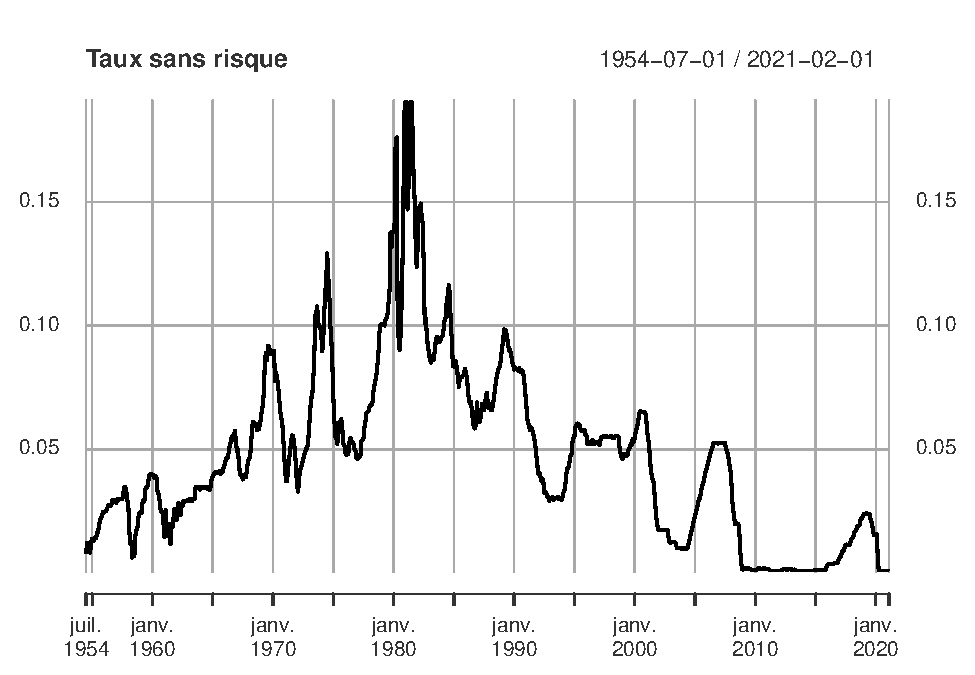
\includegraphics{TP-7-v2_files/figure-latex/unnamed-chunk-4-1.pdf}

En suivant l'exemple donné dans la vignette ``Risk Parity Portfolio,''
effectuer une simulation des stratégies suivantes, et commentez les
résultats.

\begin{Shaded}
\begin{Highlighting}[]
\NormalTok{ret }\OtherTok{\textless{}{-}} \FunctionTok{diff}\NormalTok{(}\FunctionTok{log}\NormalTok{(weekly.price))[}\SpecialCharTok{{-}}\DecValTok{1}\NormalTok{]}
\NormalTok{cov.mat }\OtherTok{\textless{}{-}} \FunctionTok{cov}\NormalTok{(ret)}
\NormalTok{mu }\OtherTok{\textless{}{-}} \FunctionTok{colMeans}\NormalTok{(ret)}
\NormalTok{N }\OtherTok{\textless{}{-}} \FunctionTok{length}\NormalTok{(}\FunctionTok{colnames}\NormalTok{(ret))}
\end{Highlighting}
\end{Shaded}

\begin{itemize}
\tightlist
\item
  \(1/N\)
\end{itemize}

\begin{Shaded}
\begin{Highlighting}[]
\NormalTok{w.ewp }\OtherTok{\textless{}{-}} \FunctionTok{rep}\NormalTok{(}\DecValTok{1}\SpecialCharTok{/}\FunctionTok{nrow}\NormalTok{(cov.mat), }\FunctionTok{nrow}\NormalTok{(cov.mat))}
\NormalTok{w.mat.ewp }\OtherTok{\textless{}{-}} \FunctionTok{matrix}\NormalTok{(}\AttributeTok{nrow=}\DecValTok{1}\NormalTok{,}\AttributeTok{ncol=}\NormalTok{N,}\AttributeTok{data =}\NormalTok{ w.ewp)}
\FunctionTok{colnames}\NormalTok{(w.mat.ewp) }\OtherTok{=} \FunctionTok{colnames}\NormalTok{(weekly.price)}
\FunctionTok{barplotPortfolioRisk}\NormalTok{(w.mat.ewp[}\DecValTok{1}\NormalTok{,], cov.mat, }\AttributeTok{col =} \StringTok{"\#A29BFE"}\NormalTok{)}
\end{Highlighting}
\end{Shaded}

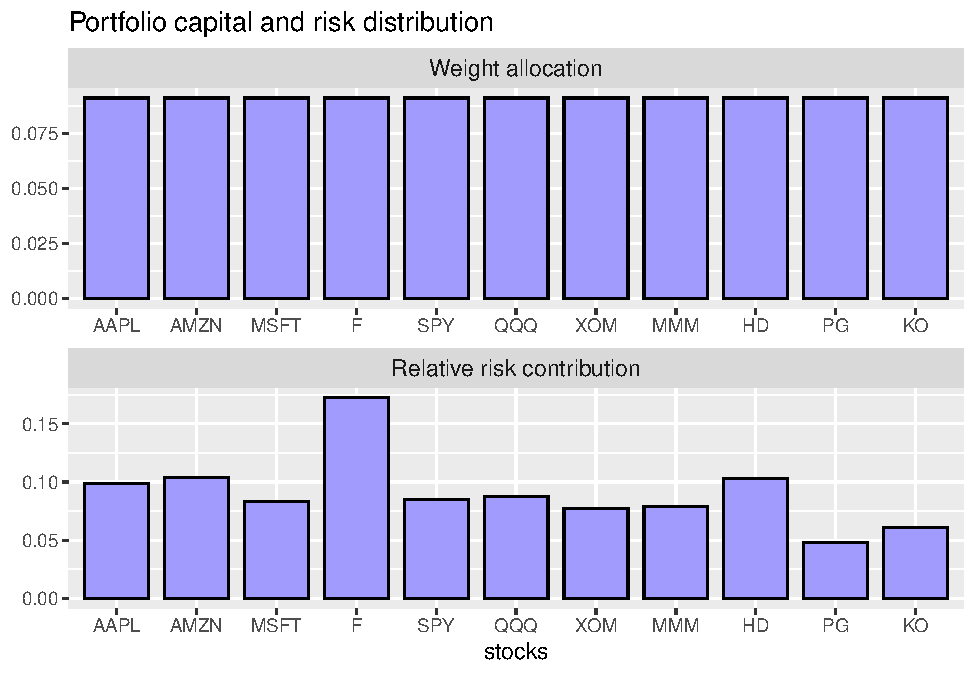
\includegraphics{TP-7-v2_files/figure-latex/unnamed-chunk-6-1.pdf} On
peut donc voir que tous les poids sont égaux contrairement à la
contribution au risque qui est plus ou moins élevée selon les titres. Un
des atouts de ce modèle est la diversification du portefeuille.

\begin{itemize}
\tightlist
\item
  Portefeuille tangent
\end{itemize}

\begin{Shaded}
\begin{Highlighting}[]
\NormalTok{max.sharpe.ratio }\OtherTok{\textless{}{-}} \ControlFlowTok{function}\NormalTok{(data) \{}
\NormalTok{    prices }\OtherTok{\textless{}{-}}\NormalTok{ data}
\NormalTok{    log.ret }\OtherTok{\textless{}{-}} \FunctionTok{diff}\NormalTok{(}\FunctionTok{log}\NormalTok{(prices))[}\SpecialCharTok{{-}}\DecValTok{1}\NormalTok{]}
\NormalTok{    N }\OtherTok{\textless{}{-}} \FunctionTok{ncol}\NormalTok{(prices)}
\NormalTok{    Sigma }\OtherTok{\textless{}{-}} \FunctionTok{cov}\NormalTok{(log.ret)}
\NormalTok{    mu }\OtherTok{\textless{}{-}} \FunctionTok{colMeans}\NormalTok{(log.ret)}
    \ControlFlowTok{if}\NormalTok{ (}\FunctionTok{all}\NormalTok{(mu }\SpecialCharTok{\textless{}=} \FloatTok{1e{-}8}\NormalTok{))}
        \FunctionTok{return}\NormalTok{(}\FunctionTok{rep}\NormalTok{(}\DecValTok{0}\NormalTok{, N))}
\NormalTok{    Dmat }\OtherTok{\textless{}{-}} \DecValTok{2} \SpecialCharTok{*}\NormalTok{ Sigma}
\NormalTok{    Amat }\OtherTok{\textless{}{-}} \FunctionTok{diag}\NormalTok{(N)}
\NormalTok{    Amat }\OtherTok{\textless{}{-}} \FunctionTok{cbind}\NormalTok{(mu, Amat)}
\NormalTok{    bvec }\OtherTok{\textless{}{-}} \FunctionTok{c}\NormalTok{(}\DecValTok{1}\NormalTok{, }\FunctionTok{rep}\NormalTok{(}\DecValTok{0}\NormalTok{, N))}
\NormalTok{    dvec }\OtherTok{\textless{}{-}} \FunctionTok{rep}\NormalTok{(}\DecValTok{0}\NormalTok{, N)}
\NormalTok{    res }\OtherTok{\textless{}{-}} \FunctionTok{solve.QP}\NormalTok{(}\AttributeTok{Dmat =}\NormalTok{ Dmat, }\AttributeTok{dvec =}\NormalTok{ dvec, }\AttributeTok{Amat =}\NormalTok{ Amat, }\AttributeTok{bvec =}\NormalTok{ bvec, }\AttributeTok{meq =} \DecValTok{1}\NormalTok{)}
\NormalTok{    w }\OtherTok{\textless{}{-}}\NormalTok{ res}\SpecialCharTok{$}\NormalTok{solution}
    \FunctionTok{return}\NormalTok{(w}\SpecialCharTok{/}\FunctionTok{sum}\NormalTok{(w))}
\NormalTok{\}}

\NormalTok{w.tangent }\OtherTok{\textless{}{-}} \FunctionTok{max.sharpe.ratio}\NormalTok{(weekly.price)}
\NormalTok{w.mat }\OtherTok{\textless{}{-}} \FunctionTok{matrix}\NormalTok{(}\AttributeTok{nrow=}\DecValTok{1}\NormalTok{,}\AttributeTok{ncol=}\NormalTok{N,}\AttributeTok{data =}\NormalTok{ w.tangent)}
\FunctionTok{colnames}\NormalTok{(w.mat) }\OtherTok{=} \FunctionTok{colnames}\NormalTok{(weekly.price)}
\FunctionTok{barplotPortfolioRisk}\NormalTok{(w.mat[}\DecValTok{1}\NormalTok{,], cov.mat, }\AttributeTok{col =} \StringTok{"\#A29BFE"}\NormalTok{)}
\end{Highlighting}
\end{Shaded}

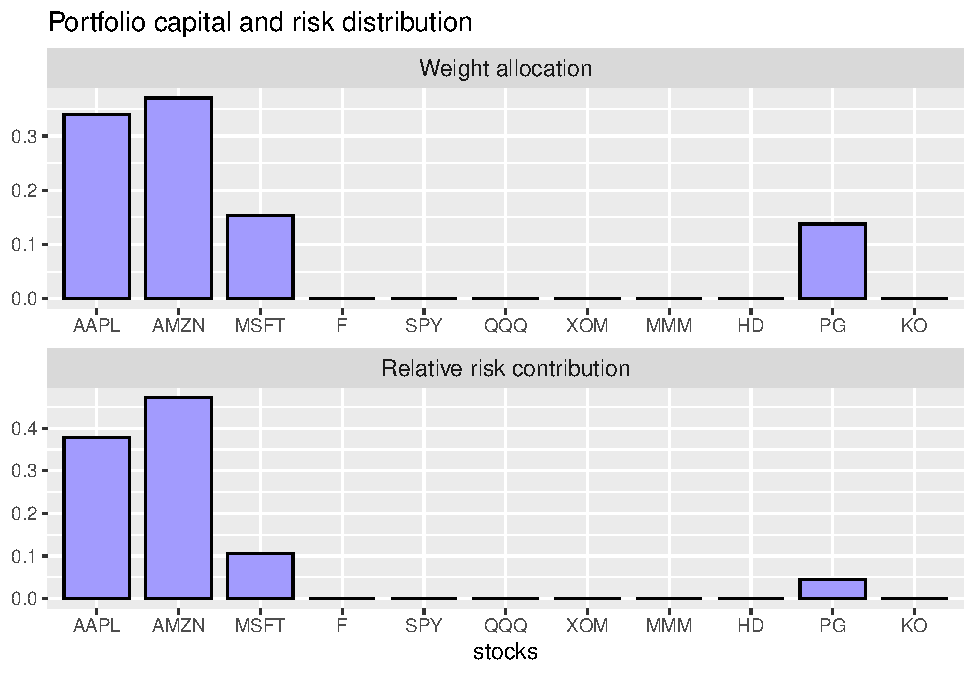
\includegraphics{TP-7-v2_files/figure-latex/unnamed-chunk-7-1.pdf} Le
portefeuille tangent alloue la richesse aux actifs à partir d'un
problème d'optimisation (cf question 1) en considérant uniquement les
risques et les rendements. Sur le diagramme, on observe une
concentration de la richesse pour seulement 4 titres : Microsoft,
Amazon, Apple et PG. Cela engendre donc peu de diversification et ainsi
un risque de corrélation sur le portefeuille.

\begin{itemize}
\tightlist
\item
  Portefeuille ``risk parity''
\end{itemize}

\begin{Shaded}
\begin{Highlighting}[]
\NormalTok{rpp }\OtherTok{\textless{}{-}} \FunctionTok{riskParityPortfolio}\NormalTok{(cov.mat)}
\FunctionTok{barplotPortfolioRisk}\NormalTok{(rpp}\SpecialCharTok{$}\NormalTok{w, cov.mat, }\AttributeTok{col =} \StringTok{"\#A29BFE"}\NormalTok{)}
\end{Highlighting}
\end{Shaded}

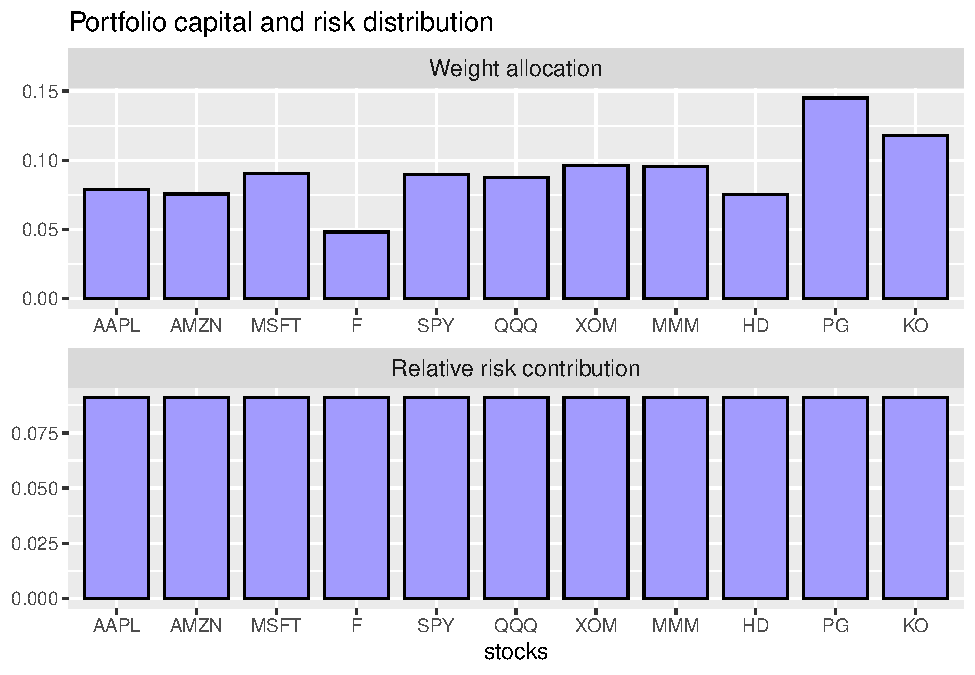
\includegraphics{TP-7-v2_files/figure-latex/unnamed-chunk-8-1.pdf} La
stratégie RiskParityPortfolio attribue le même risque à tous les actifs.
Cependant, on remarque également que tous les actifs ont un poids
significatif dans le portefeuille, à l'encontre par exemple du
portefeuille tangent précédent.

\hypertarget{question-3-comparaison-de-diverses-stratuxe9gies-dallocation-avec-contraintes-de-diversification}{%
\section{Question 3: Comparaison de diverses stratégies d'allocation,
avec contraintes de
diversification}\label{question-3-comparaison-de-diverses-stratuxe9gies-dallocation-avec-contraintes-de-diversification}}

Ajoutez les contraintes suivantes aux portefeuilles ``risk parity'' et
``tangent,'' et exécutez les simulations de gestion. Comparez ces
résultats aux simulations de la question 2.

\[
\begin{aligned}
w_i & \leq 25\% \\
w_{AAPL} + w_{MSFT} + w_{AMZN} & \leq 40\%
\end{aligned}
\] 1) Portefeuille tangent

\begin{Shaded}
\begin{Highlighting}[]
\NormalTok{max.sharpe.ratio}\FloatTok{.2} \OtherTok{\textless{}{-}} \ControlFlowTok{function}\NormalTok{(data) \{}
\NormalTok{    prices }\OtherTok{\textless{}{-}}\NormalTok{ data}
\NormalTok{    log.ret }\OtherTok{\textless{}{-}} \FunctionTok{diff}\NormalTok{(}\FunctionTok{log}\NormalTok{(prices))[}\SpecialCharTok{{-}}\DecValTok{1}\NormalTok{]}
\NormalTok{    N }\OtherTok{\textless{}{-}} \FunctionTok{ncol}\NormalTok{(prices)}
\NormalTok{    Sigma }\OtherTok{\textless{}{-}} \FunctionTok{cov}\NormalTok{(log.ret)}
\NormalTok{    mu }\OtherTok{\textless{}{-}} \FunctionTok{colMeans}\NormalTok{(log.ret)}
    \ControlFlowTok{if}\NormalTok{ (}\FunctionTok{all}\NormalTok{(mu }\SpecialCharTok{\textless{}=} \FloatTok{1e{-}8}\NormalTok{))}
        \FunctionTok{return}\NormalTok{(}\FunctionTok{rep}\NormalTok{(}\DecValTok{0}\NormalTok{, N))}
\NormalTok{    Dmat }\OtherTok{\textless{}{-}} \DecValTok{2} \SpecialCharTok{*}\NormalTok{ Sigma}
\NormalTok{    Amat }\OtherTok{\textless{}{-}} \SpecialCharTok{{-}}\FunctionTok{diag}\NormalTok{(N)}
\NormalTok{    Amat }\OtherTok{\textless{}{-}} \FunctionTok{cbind}\NormalTok{(mu,Amat)}
\NormalTok{    Amat }\OtherTok{\textless{}{-}} \FunctionTok{cbind}\NormalTok{(Amat,}\FunctionTok{c}\NormalTok{(}\FunctionTok{rep}\NormalTok{(}\SpecialCharTok{{-}}\DecValTok{1}\NormalTok{,}\DecValTok{3}\NormalTok{),}\FunctionTok{rep}\NormalTok{(}\DecValTok{0}\NormalTok{,}\DecValTok{8}\NormalTok{)))}
\NormalTok{    bvec }\OtherTok{\textless{}{-}} \FunctionTok{c}\NormalTok{(}\FloatTok{0.005}\NormalTok{, }\FunctionTok{rep}\NormalTok{(}\SpecialCharTok{{-}}\FloatTok{0.25}\NormalTok{, N),}\SpecialCharTok{{-}}\FloatTok{0.4}\NormalTok{)}
\NormalTok{    dvec }\OtherTok{\textless{}{-}} \FunctionTok{rep}\NormalTok{(}\DecValTok{0}\NormalTok{, N)}
\NormalTok{    res }\OtherTok{\textless{}{-}} \FunctionTok{solve.QP}\NormalTok{(}\AttributeTok{Dmat =}\NormalTok{ Dmat, }\AttributeTok{dvec =}\NormalTok{ dvec, }\AttributeTok{Amat =}\NormalTok{ Amat, }\AttributeTok{bvec =}\NormalTok{ bvec, }\AttributeTok{meq =} \DecValTok{1}\NormalTok{)}
\NormalTok{    w }\OtherTok{\textless{}{-}}\NormalTok{ res}\SpecialCharTok{$}\NormalTok{solution}
    \FunctionTok{return}\NormalTok{(w}\SpecialCharTok{/}\FunctionTok{sum}\NormalTok{(w))}
\NormalTok{\}}

\NormalTok{w.tangent}\FloatTok{.2} \OtherTok{\textless{}{-}} \FunctionTok{max.sharpe.ratio.2}\NormalTok{(weekly.price)}
\NormalTok{w.mat}\FloatTok{.2} \OtherTok{\textless{}{-}} \FunctionTok{matrix}\NormalTok{(}\AttributeTok{nrow=}\DecValTok{1}\NormalTok{,}\AttributeTok{ncol=}\NormalTok{N,}\AttributeTok{data =}\NormalTok{ w.tangent}\FloatTok{.2}\NormalTok{)}
\FunctionTok{colnames}\NormalTok{(w.mat}\FloatTok{.2}\NormalTok{) }\OtherTok{\textless{}{-}} \FunctionTok{colnames}\NormalTok{(weekly.price)}
\FunctionTok{barplotPortfolioRisk}\NormalTok{(w.mat}\FloatTok{.2}\NormalTok{[}\DecValTok{1}\NormalTok{,], cov.mat, }\AttributeTok{col =} \StringTok{"\#A29BFE"}\NormalTok{)}
\end{Highlighting}
\end{Shaded}

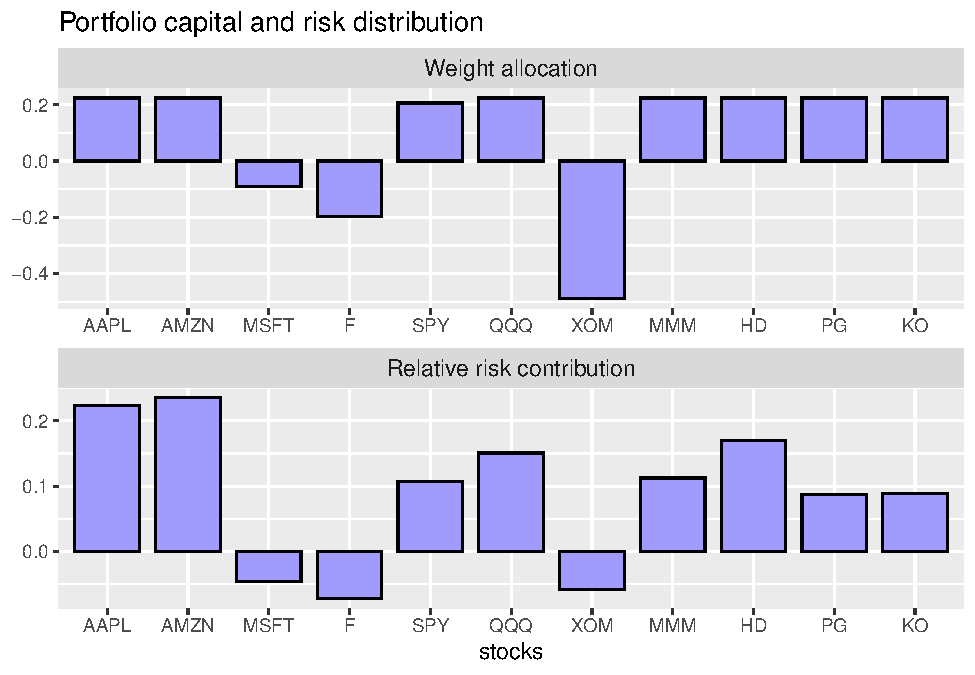
\includegraphics{TP-7-v2_files/figure-latex/unnamed-chunk-9-1.pdf} On
obtient bien comme résultat un portefeuille où tous les poids sont
inférieurs à 25\% et où la somme des poids de Amazon, Apple et Microsoft
est inférieure à 40\%. Le portefeuille obtenu est ainsi beaucoup plus
diversifié que le précédent portefeuille tangent.

\begin{enumerate}
\def\labelenumi{\arabic{enumi})}
\setcounter{enumi}{1}
\tightlist
\item
  Risk Parity Portfolio
\end{enumerate}

\begin{Shaded}
\begin{Highlighting}[]
\NormalTok{Amat }\OtherTok{\textless{}{-}} \SpecialCharTok{{-}}\FunctionTok{diag}\NormalTok{(N)}
\NormalTok{Amat }\OtherTok{\textless{}{-}} \FunctionTok{cbind}\NormalTok{(mu,Amat)}
\NormalTok{Amat }\OtherTok{\textless{}{-}} \FunctionTok{cbind}\NormalTok{(Amat,}\FunctionTok{c}\NormalTok{(}\FunctionTok{rep}\NormalTok{(}\SpecialCharTok{{-}}\DecValTok{1}\NormalTok{,}\DecValTok{3}\NormalTok{),}\FunctionTok{rep}\NormalTok{(}\DecValTok{0}\NormalTok{,}\DecValTok{8}\NormalTok{)))}

\CommentTok{\#rpp.2 \textless{}{-} riskParityPortfolio(cov.mat, Dmat = Amat, dvec = c(0.005, rep({-}0.25, N),{-}0.4))}
\CommentTok{\#ncol(Amat)}
\CommentTok{\#length(c(0.005, rep({-}0.25, N),{-}0.4))}
\CommentTok{\#barplotPortfolioRisk(rpp.2$w, cov.mat, col = "\#A29BFE")}
\end{Highlighting}
\end{Shaded}

Nous n'avons pas réussi à finaliser le code pour le Risk Parity
Portfolio en ajoutant les matrices de contraintes d'inégalité à la
fonction riskParityPortfolio de R.

\end{document}
